\section{Design}

\subsection{Event}
An event is represented by a rounded rectangle with a short text inside summarizing its content. The width of an event rectangle is constrained by some maximum value and long text is trimmed to fit into its area. The full content of an event will be displayed when it is hovered. Events can be classified into different categories based on a certain criteria. For example, a news article may write about \emph{sport}, \emph{fashion} or both. Small colored badges are added to the left of the text of an event to indicate its categories. The colors are chosen from Qualitative Set 1 of  ColorBrewer~\cite{Harrower2003}. Only around 12 colors can be distinguished simultaneously in the human view~\cite{Munzner2014}. Therefore, only the eight most frequently appeared categories are displayed using the selected colormap; whereas, the rest share a different color. Figure~\ref{fig:event} shows an event with three categories.

\begin{figure}[!htb]
\centering
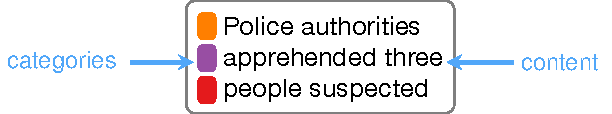
\includegraphics{event}
\caption{Visual representation of event. Text shows the content and colored badges indicate the categories.}
\label{fig:event}
\end{figure}

An event is left-aligned with its temporal value on the time axis. To reduce cluttering, an event is not visually connected to its corresponding point on the axis. Instead, it only appears when the event is hovered. The time axis is shown as a horizontal line at the bottom of all events. It includes two hierarchical temporal scales, changed dynamically according to the range of the visible events. For example, the time axis in Figure~\ref{fig:sl-overview} shows \emph{month} and \emph{day} but they can be switched to \emph{year} and \emph{month} if needed to cover the range of events.

\subsection{Schema}
As discussed in Section~\note{ref}, Gestalt principles of grouping are commonly used to show relationships between events, most effectively \emph{connectedness} and \emph{proximity}. Therefore, we also apply these two principles in our design: events belonging to the same schema are located close together; and the background of the entire schema is colored to visually connected all of its events. Spatial grouping needs to be achieved through vertical positioning because the horizontal position of each event is already determined by its temporal information. Locating all events within a schema close together also makes it convenient to follow them chronologically (Requirement 2).

Munroe's hand-drawn movie narrative charts~\cite{Munroe2009} show the dynamic interactions of characters throughout the movie. Each character is represented as a curved line along a horizontal time axis; and vertical grouping of lines indicates which characters are together at a given interval. Inspired by this technique, we consider a ``schema'' as a ``character line'', connecting all of its events. However, instead of a thin line, we use a thicker path to provide enough space for displaying the content of events and to allow convenient interaction with individual events. For aesthetics, the path is connected rectilinearly, including only horizontal and vertical segments. Also,  all events are constrained by the same height to make the width of the path consistent. Figure~\ref{fig:schema} shows two examples of schema. 

\begin{figure}[!htb]
	\centering
	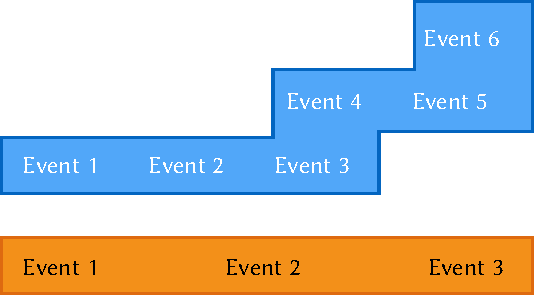
\includegraphics{schema}
	\caption{Visual representation of schema as a colored stripe. Bottom: a simple rectangle connects events that can display in the same row. Top: a rectilinear path connects events that need to locate in different rows.}
	\label{fig:schema}
\end{figure}

Putting it all together, Figure~\ref{fig:sl-overview} shows an example of a complete SchemaLine visualization. The algorithm to produce this is described in Section~\ref{sec:sl-algorithm}.

\begin{figure}[!htb]
	\centering
	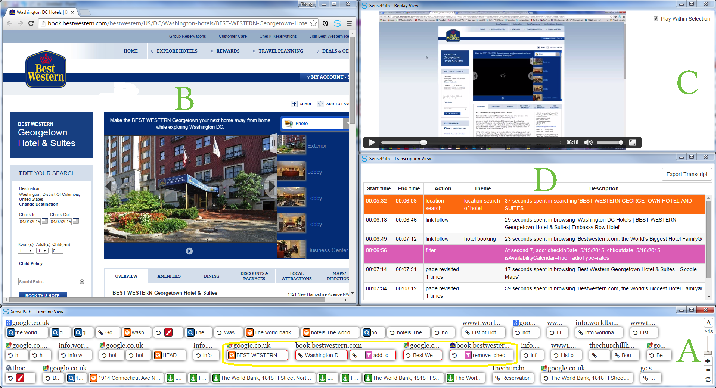
\includegraphics[width=\linewidth]{overview}
	\caption{SchemaLine visualization of user annotations. Related notes are connected to form schemas.}
	\label{fig:sl-overview}
\end{figure}

\subsection{Interaction}
To enable users to intuitively perform sensemaking activities described in the Data--Frame model (Requirement 3), we follow the design guidelines proposed by Elmqvist~et~al.~\cite{Elmqvist2011} for fluid interaction. More specifically, SchemaLine uses smooth animated transitions between states, provides immediate visual feedback on interaction, and uses direct manipulation of visual representations.

Sensemaking activities in Data-Frame model involve two different types of entities: \textit{data} and \textit{frame}. We allow direct manipulation of visual representations of data and frame, instead of invoking menus and buttons to perform actions. The first sensemaking activity in the Data-Frame model is to \textbf{construct a new frame} by connecting relevant data. It can be performed in SchemaLine by \textit{dragging one event and dropping it onto another event}. A \textit{plus} icon and a \textit{dashed rectangle} surrounding the two events are displayed to indicate that a new frame will be created. When dropping the event, a color stripe representing a frame will be formed by connecting these two events, and a smooth animated transition is used to improve user perception.

Besides dropping an event on top of another event, the user can drop it onto the color stripe to add that event to an existing frame (\textbf{elaborate a frame}). Conversely, the user can drag an event belonging to a frame and drop it onto the void space to remove it from the frame (\textbf{preserving a frame}). Appropriate informative feedback is displayed, \textit{plus} icon for addition and \textit{minus} icon for subtraction, and a smooth animated transition is used to improve user perception. Fig.~\ref{fig:drag-drop-note} shows an example of adding an event into a frame.
\begin{figure}[!htb]
	\centering
	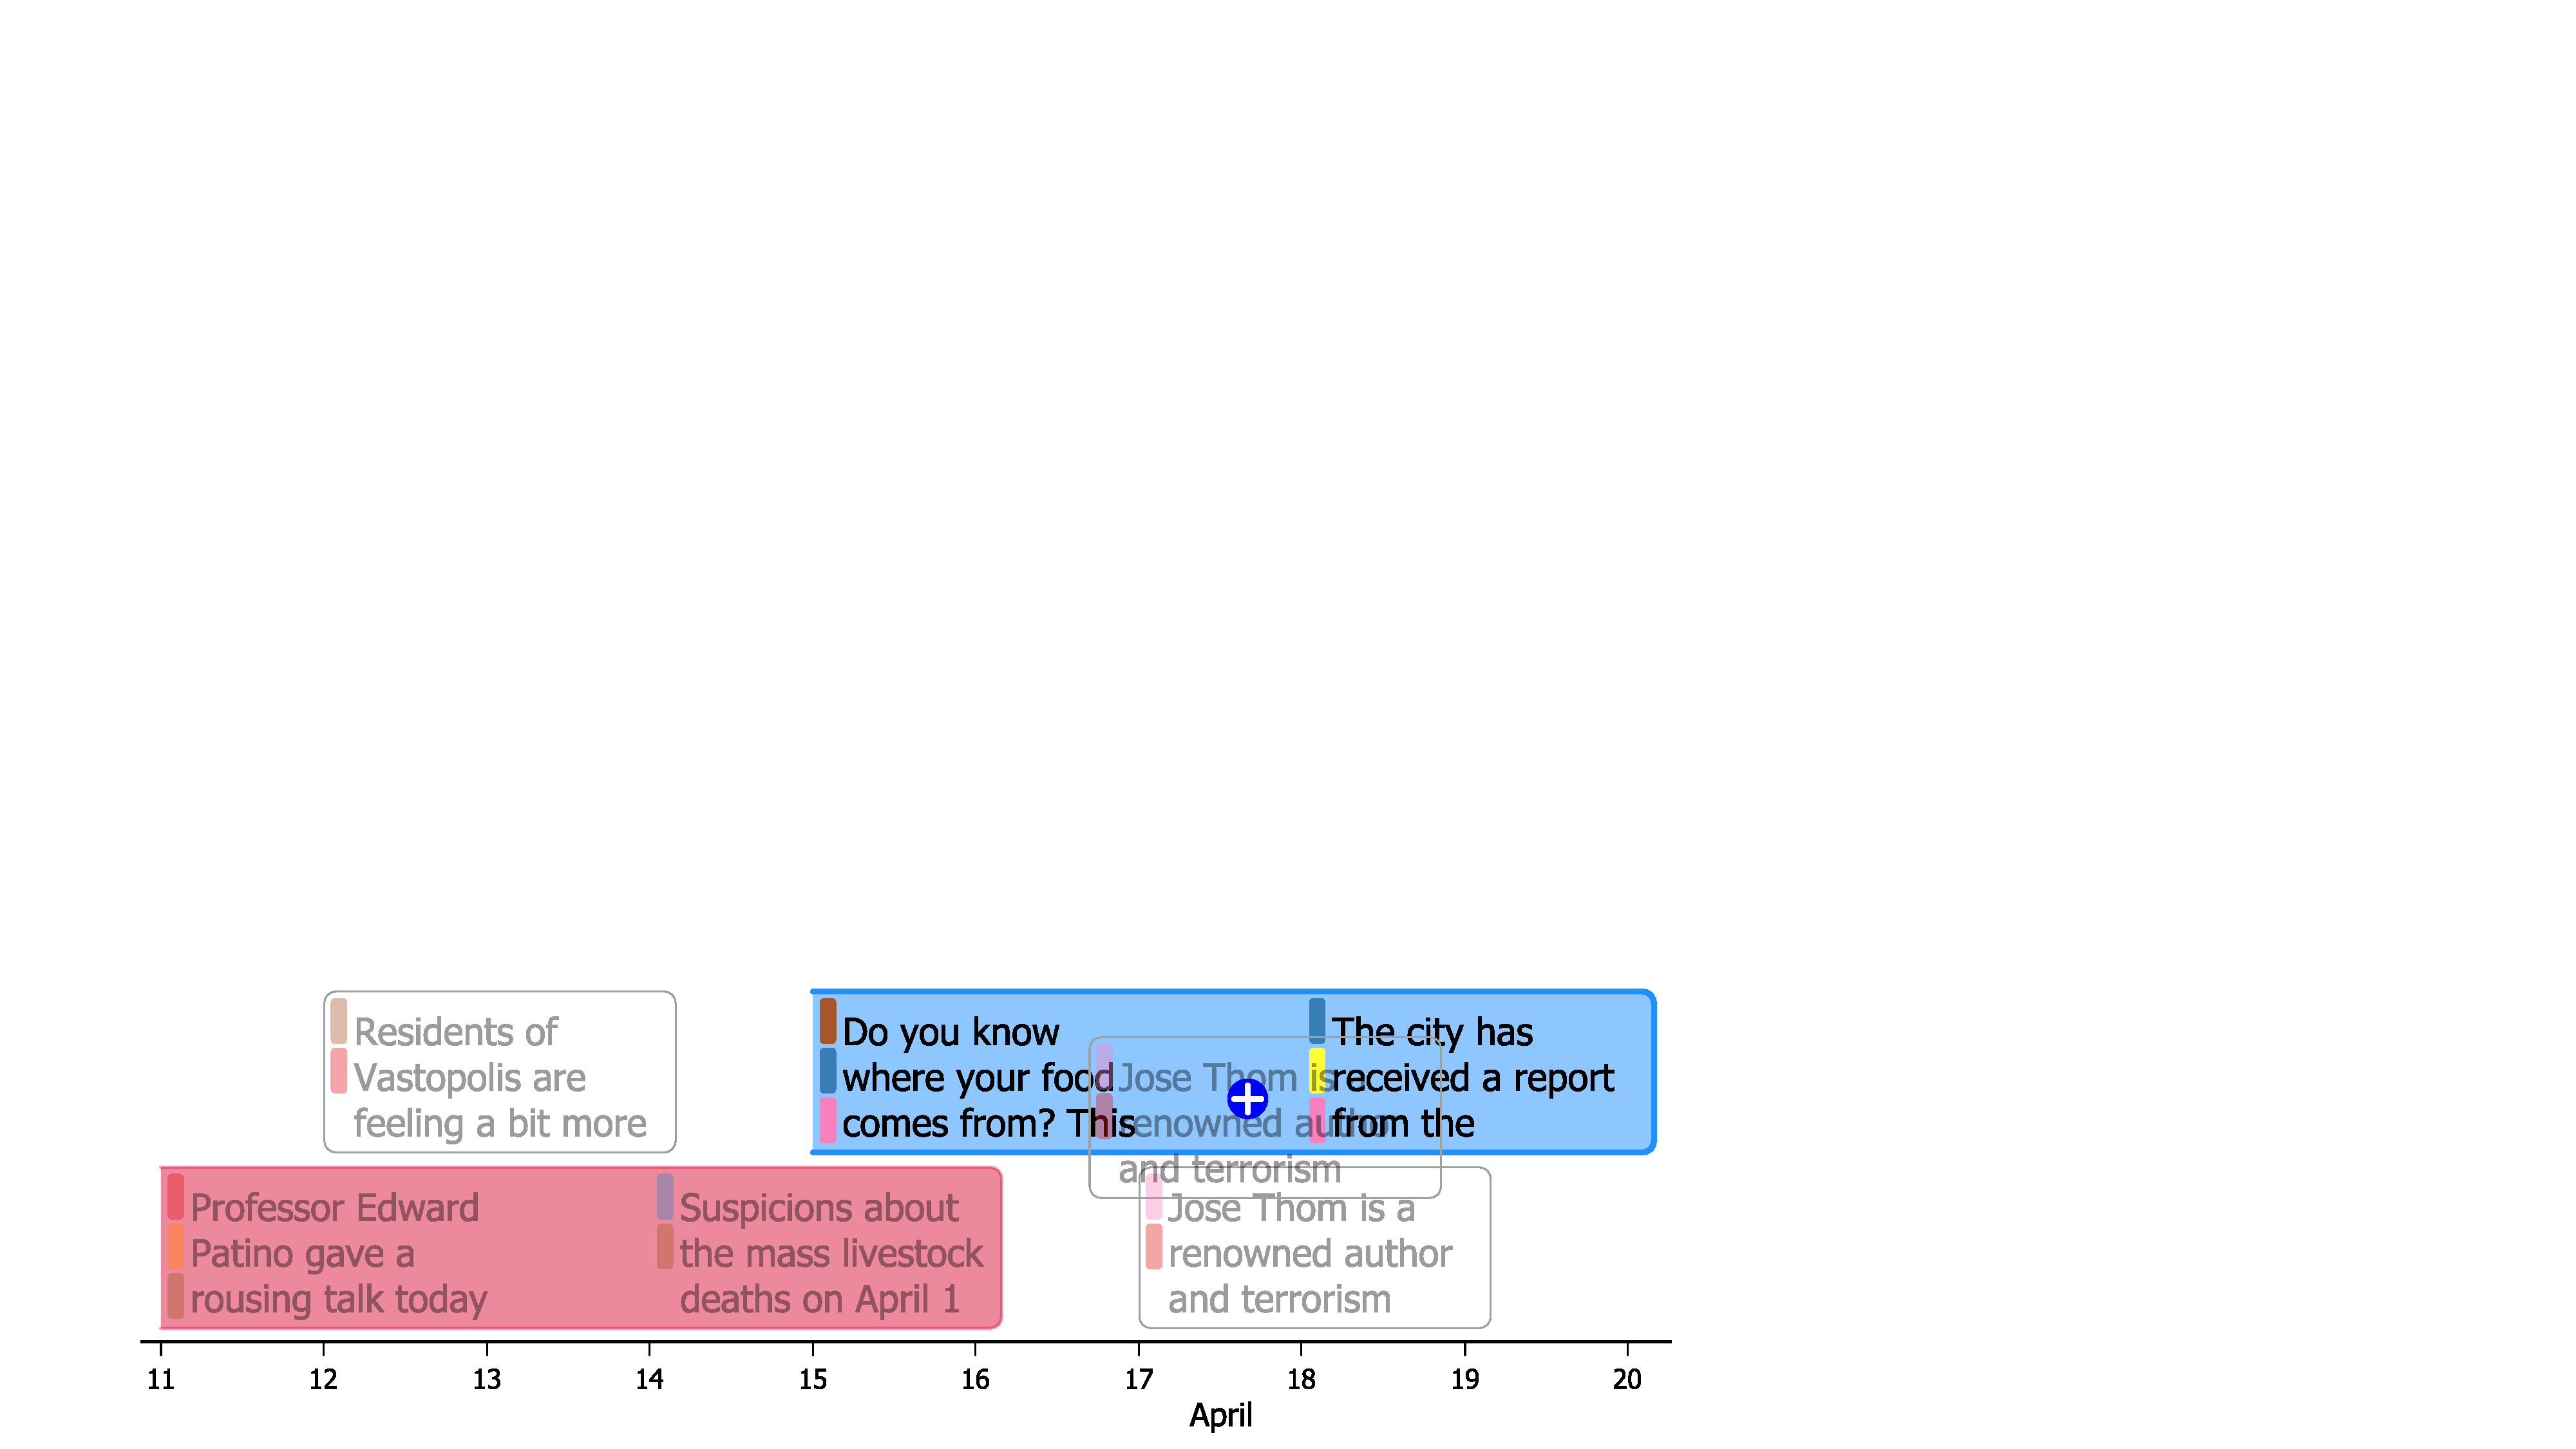
\includegraphics[width=.9\linewidth]{add-event-frame}
	\caption{Elaborating a frame. Dragging and dropping an event onto the blue stripe to add it to the frame.}
	\label{fig:drag-drop-note}
\end{figure}



\textbf{Questioning a frame} occurs when the user encounters inconsistencies in data within a frame. The temporal distribution of events in the frame may suggest some concerns about the validity or completeness of the frame. For example, if a frame about one person contains many events in January and March, but no events are found in February, then it may be inferred that there could be some data missing. The analyst can mark a suspected event by right-mouse double-clicking on it. Red color text is used to indicate that the event needs more investigation. 

Dragging an event from one frame to another frame will remove it from the old frame and add it to the new frame. However, holding \textit{Control} key when dropping will instead copy the event to the new frame. This interaction allows the analyst to duplicate events to create several similar frames and compare them (\textbf{comparing frames}). When two frames are selected, they will be moved closer together to allow easy comparison, irrespective of the frames ordering generated by the layout algorithm. The user can drag an entire frame and drop it onto another frame to merge all events together. The user can also drop the frame onto the void space to take apart the frame and release its events. This interaction is useful when the user thinks that the frame is completely wrong and wants to construct a new frame (\textbf{reframing}).

Other interactions with events are also designed to be intuitive. Left-mouse double-clicking on an event opens its full content. Dragging an event with the right mouse button can change the event's date. This feature is useful because the report date is not always the date when the event actually occurred; for example, ``yesterday there was a bomb attack in ABC''. Dragging an event outside the boundary of the timeline will remove it from the system (with \textit{remove} icon as informative feedback).

Once any change is made on SchemaLine, such as moving an event from one frame to another, an animation is shown of smooth transition between the changes to help analyst update their ``mental map''. To achieve this, the layout algorithm (Section \ref{sub:schema-layout}) computes the new event rectangle locations. Then, the outline algorithm (Section \ref{sub:schema-outline}) runs at every step of the interpolation between the old and the new locations to produce intermediate polygon paths based on the updated event locations.